\documentclass{article}

\usepackage[left=3cm,right=3cm,top=2cm,bottom=2cm]{geometry}
\usepackage{xetexko}
\usepackage{listing}
\usepackage{graphicx}

\begin{document}
    \title{<컴퓨터 프로그래밍 3> 실습보고서 \\ \large [제 02 주] 이차방정식}
    \date{\today}
    \author{201704150 허강준}

    \maketitle

    \newpage

    \tableofcontents

    \newpage

    \section{프로그램 명세}

    \subparagraph{\normalfont본 실습 보고서는 <컴퓨터 프로그래밍 3> 강의의 제 02주차 실습 과제인 이차 방정식 프로그램의 구현과 그 실행 결과의 분석에 대해 다룬다.}

    \subsection{설계}

    \subparagraph{\normalfont이전 과제인 <일차 방정식> 프로그램의 상당 부분을 재활용하였다. 대신 이차방정식 처리를 위하여 \texttt{QuadEquation} 모듈을 추가하였다.}

    \subsection{함수 명세}

    \subparagraph{\normalfont모든 프로시져들은 리턴 형 (\texttt{void})를 생략한다.}

    \paragraph{\large\texttt{int main(void)} \tiny Main.c, Ln 10}

    \subparagraph{\normalfont프로그램의 진입점이다. \texttt{App\_Start}를 호출한다.}

    \paragraph{\large\texttt{int App\_Start(void)} \tiny App.h, Ln 9}

    \subparagraph{\normalfont\texttt{App} 모듈의 진입점이다. 모든 동작은 이 안에서 실행된다.}
    
    \paragraph{\large\texttt{AppView\_out\_msg\_startSolvingQuadEquation(void)} \tiny AppView.h, Ln 9}

    \subparagraph{\normalfont\texttt{<<< 이차방정식 풀이를 시작합니다 >>>} 라는 메세지를 출력한다. \texttt{App} 모듈 시작 시 호출된다.}

    \paragraph{\large\texttt{AppView\_out\_msg\_endSolvingQuadEquation(void)} \tiny AppView.h, Ln 10}

    \subparagraph{\normalfont\texttt{<<< 이차방정식 풀이를 종료합니다 >>>} 라는 메세지를 출력한다. \texttt{App} 모듈 종료 시 호출된다.}

    \paragraph{\large\texttt{AppView\_out\_showQuadEquation(QuadEquationProblem\_t problem)} \tiny AppView.h, Ln 11}
    
    \subparagraph{\normalfont \texttt{QuadEquationProblem\_t} 객체를 인자로 받아 현재 입력된 이차방정식을 출력한다.}

    \paragraph{\large\texttt{AppView\_out\_showRoot(float root)} \tiny AppView.h, Ln 12}

    \subparagraph{\normalfont 인자로 제공된 \texttt{QuadEquationProblem\_t} 객체에 저장된 이차방정식의 해를 출력한다.}

    \paragraph{\large\texttt{AppView\_out\_msg\_error\_secondOrderTermCoefficientIsZero(void)} \tiny AppView.h, Ln 13}

    \subparagraph{\normalfont 2차항의 계수가 0이기 때문에 이차방정식이 성립할 수 없다는 오류메세지를 출력한다.}

    \paragraph{\large\texttt{AppView\_out\_msg\_error\_determinantIsNegative(QuadEquationProblem\_t problem)} \tiny AppView.h, Ln 14}

    \subparagraph{\normalfont 이차방정식의 판별식이 음수이므로 해를 내놓을 수 없다는 에러와 해당 판별식 결과값을 출력한다.}

    \paragraph{\large\texttt{bool AppView\_in\_getSolvingRequest(void)} \tiny AppView.h, Ln 16}

    \subparagraph{\normalfont 사용자로부터 방정식을 풀 것인지 묻는 메세지를 출력하여 입력을 받는다. \texttt{y} 나 \texttt{Y}를 입력받을 경우 \texttt{true}를, 그 외의 경우 \texttt{false}를 리턴한다.}

    \paragraph{\large\texttt{AppView\_in\_getCoefficient(QuadEquationProblem\_t*)} \tiny AppView.h, Ln 17}

    \subparagraph{\normalfont 사용자로부터 계수로 사용할 두개 값을 입력받는다. 이때 저장은 인자로 전달받은 두개의 \texttt{float} 포인터를 통해 저장한다.}

    \paragraph{\large\texttt{QuadEquationProblem\_setEquation(QuadEquationProblem\_t* \_this, QuadEquation\_t equation)} \tiny QuadEquation.h, Ln 20}

    \subparagraph{\normalfont \texttt{QuadEquation\_t} 객체를 받아 \texttt{\_this->equation}을 변경한다. }

    \paragraph{\large\texttt{bool QuadEquationProblem\_secondOrderTermCofficientIsZero(QuadEquationProblem\_t* \_this)} \tiny QuadEquation.h, Ln 21}

    \subparagraph{\normalfont 2차항의 계수가 0인지 검사하는 메서드이다. 0일 경우 \texttt{true}를 반환한다.}

    \paragraph{\large\texttt{bool QuadEquationProblem\_determinantIsNegative(QuadEquationProblem\_t* \_this)} \tiny QuadEquation.h, Ln 22}

    \subparagraph{\normalfont 판별식이 음수인지 검사하는 메서드이다. 음수일 경우 \texttt{true}를 반환한다.}

    \paragraph{\large\texttt{float QuadEquationProblem\_getDeterminant(QuadEquationProblem\_t* \_this)} \tiny QuadEquation.h, Ln 23}

    \subparagraph{\normalfont 판별식을 계산하여 반환하는 메서드이다.}

    \paragraph{\large\texttt{QuadEquationProblem\_solve(QuadEquationProblem\_t* \_this)} \tiny QuadEquation.h, Ln 24}

    \subparagraph{\normalfont \texttt{\_this->equation} 객체에 저장된 값을 바탕으로 해를 계산한 뒤 \texttt{\_this->solution}에 저장한다.}


    \paragraph{MACRO \large\texttt{Square(x)} \tiny Macros.h, Ln 6}

    \subparagraph{\normalfont제곱값 매크로이다.}

    \paragraph{MACRO \large\texttt{F32Abs(f0)} \tiny Macros.h, Ln 8}

    \subparagraph{\normalfont인자로 전달된 32비트 부동소수점 값의 절댓값을 산출한다. IEEE-754에 정의된 단정밀도 부동소숫점의 정의에 따라, MSB의 값을 Bitwise-AND를 통하여 0으로 만든다. \\ 이때 \texttt{f0}와 Bitwise-AND 되는 operand는 \texttt{0x7fffffff}이다.}

    \paragraph{MACRO \large\texttt{F32IsZero(f0)} \tiny Macros.h, Ln 9}

    \subparagraph{\normalfont인자로 전달된 32비트 부동소수점 값의 절댓값이 0인지 검사한다. 같은 파일에서 \texttt{1.0E-6}로 정의된 \texttt{EPSILON}보다 작은지 검사한다.}

    \subsection{종합 명세}

    \subparagraph{\normalfont1주차의 일차방정식 프로그램과 전체적인 동작은 비슷하나, 2차항의 계수가 0인지 아닌지, 그리고 판별식($b^2-4ac$)이 음수인지 검사하는 부분이 추가되었다. 또힌 이차방정식 객체의 처리를 위하여 이차방정식 문제를 정의하는 \texttt{QuadEquationProblem\_t}, 이차방정식을 정의하는 \texttt{QuadEquation\_t}, 그리고 해를 정의하는 \texttt{QuadSolution\_t} 를 정의하였다.}

    \subparagraph{\normalfont객체지향적인 코드를 위하여 \texttt{QuadEquationProblem\_t} 의 포인터를 첫번째 인자 \texttt{\_this}로 받는 함수들을 정의하였으며, 이를 통해 \texttt{App\_Start}에서 \texttt{QuadEquationProblem\_t} 객체의 내부를 직접 접근하거나 변경할 필요가 없도록 하였다.}

    \section{프로그램의 장단점 및 특이점 분석}
    
    \subsection{\texttt{QuadEquationProblem\_t\*}를 인자로 받도록 한 이유}

    \subparagraph{\normalfont C에서는 Call-By-Value가 기본이며 Call-By-Reference가 존재하지 않는다. 따라서 인자로 전달된 모든 값은 복사되며 함수나 프로시져 내에서 변경하여도 원본에 영향을 미치지 않는다. 대신 포인터를 인자로 전달하여(Call-By-Address) 해당 동작을 구현해 낼 수 있다.}

    \subparagraph{\normalfont \texttt{AppView\_in\_getCoefficient}에서 그 예시를 찾아볼 수 있는데, \texttt{QuadEquation\_t} 객체의 포인터를 전달하여 내부의 계수를 수정하도록 하였다. 따라서 원본 \texttt{QuadEquation\_t} 객체를 변경할 수 있다. (사이드이펙트) 다만 이 점은 다소 아쉬운 것이, \texttt{QuadEquation\_t}의 멤버를 외부 함수가 직접 수정한다는 점에서 개선이 필요하다. 만일 개선한다면 후술할 OOP적 접근을 통해 \texttt{setCoefficient} 함수를 호출하는 식으로 수정할 수 있을 것이다.}

    \subparagraph{\normalfont 그러나 \texttt{QuadEquation} 모듈에서 정의된 함수들의 예는 조금 다른 문제로, OOP적인 코드 작성을 위해 \texttt{QuadEquationProblem\_t}의 메서드로 다루고자 하는 함수들의 첫번쨰 인자를 \texttt{QuadEquationProblem\_t}의 포인터 \texttt{\_this} 로 받도록 한 것이다. 즉, \texttt{QuadEquationProblem\_t} 타입이 가질 수 있는 동작들을 정의한 것이다.}

    \subparagraph{\normalfont 다만 C언어임에도 불구하고 \texttt{this} 를 사용하지 못한 이유는 단순히 MSVC가 C++ 컴파일러인 탓으로, \texttt{this}가 예약어이기 때문에 컴파일 오류를 일으켰기 떄문이다.}

    \subsection{판별식이 음수임을 검사할 때 \texttt{F32IsZero}를 추가한 이유}

    \subparagraph{\normalfont 부동소숫점 값은 0과 직접 비교시 의도치 못한 동작을 유발할 위험이 있다. 따라서 검사 대상 값이 0보다 작음을 검사함과 동시에 \texttt{F32IsZero}가 \texttt{false}인지 검사할 필요가 있는 것이다.}

    \section{실행 결과 분석}

    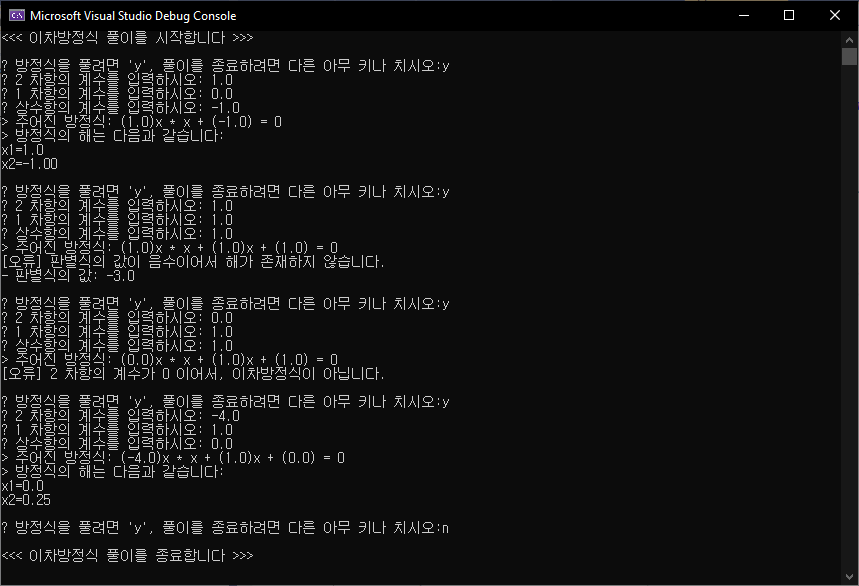
\includegraphics[width=\textwidth]{test_result.png}

    \subsection{입력과 출력}

    입력값은 실습 PPT에 제시된 예제를 따랐으며, 이에 따라 동일한 출력이 발생하였는 지를 확인하였음.

    \subsection{결과 분석}

    모든 테스트 입력과 출력에 대하여 정상임을 확인하였음. 
    
    \section{소스코드}
    전체 소스코드는 GitHub (0x00000FF/CNUCSE-Computer-Programming-III-2020-Spring) 에 업로드 되어 있으며, 제출시 본 보고서와 동봉되어 있다.
\end{document}

